\documentclass[border=4pt]{standalone}
\usepackage{tikz}
\usetikzlibrary{arrows.meta,positioning,shapes.multipart}
\begin{document}
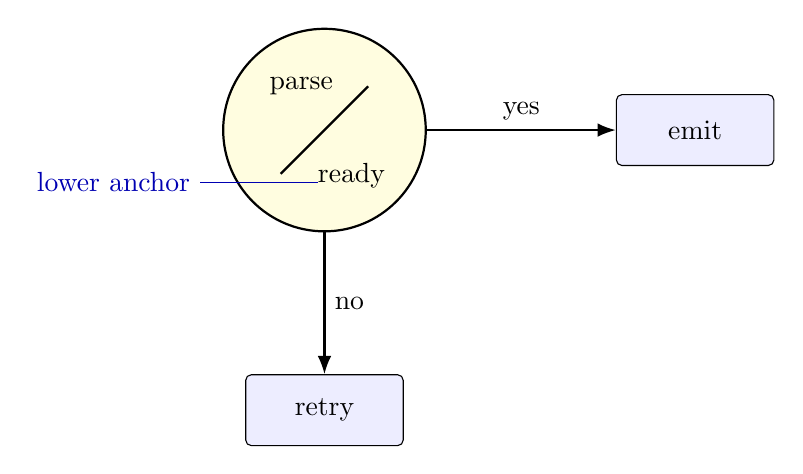
\begin{tikzpicture}[
  >=Latex,
  node distance=18mm and 24mm,
  state/.style={circle solidus,draw,thick,minimum size=24mm,
    inner xsep=5pt,inner ysep=4pt,fill=yellow!12},
  action/.style={draw,rounded corners=2pt,minimum width=20mm,
    minimum height=9mm,fill=blue!7}
]
  \node[state] (gate) {parse\nodepart{lower}ready};
  \node[action,right=of gate] (accept) {emit};
  \node[action,below=of gate] (retry) {retry};

  \draw[-Latex,thick] (gate) -- node[above] {yes} (accept);
  \draw[-Latex,thick] (gate) -- node[right] {no} (retry);
  \draw[blue!70!black] (gate.lower) -- ++(-15mm,0)
    node[left] {lower anchor};
\end{tikzpicture}
\end{document}
